\chapter{Algorithms}\label{chap:algorithms}
This thesis examines three load balancing algorithms: the Continuous Single-Proposal Deal-Agreement-Based algorithm, the Push-Pull Sum algorithm, and the proposed Adaptive Threshold Push-Pull Sum algorithm. The Adaptive Threshold Push-Pull Sums structure is described, along with how it incorporates features from the first two algorithms and the objective behind its development. The working mechanics of each algorithm are described along with pseudo-code. Furthermore, examples are provided to show how the algorithms achieve a balanced state in the network. To provide further light on the objectives of the Adaptive Threshold Push-Pull Sum method, the aspired results are described.

\section{Characteristics}\label{sec:algoCharacteristics}
Like the graphs, load balancing algorithms may have different characteristics. These characteristics are elaborated on below:

\textbf{Static and Dynamic}: Load balancing algorithms can be classified as either static or dynamic algorithms. Static algorithms assign tasks to the nodes at compile time, while dynamic algorithms assign tasks at run time. The main advantage that static load balancing algorithms have over dynamic load balancing algorithms is that they do not cause any run-time overhead. \cite{Bokhari}

\textbf{Stochastic and Deterministic}: Stochastic load balancing algorithms rely on randomness to select load transfer partners. Deterministic load balancing algorithms, on the other hand, follow predefined distribution rules in order to make load transfers. \cite{ChengzhongFrancis}

\textbf{Global and Local}: Local load balancing algorithms allow nodes to transfer loads within their neighborhood, while global load balancing algorithms enable load balancing operations across the entire network \cite{ChengzhongFrancis}.

\textbf{Monotonic and Non-monotonic}: An algorithm is considered monotonic if each load transfer is from a higher-loaded node to a less-loaded node and the maximal load in the network never increases and the minimal load never decreases \cite{Dinitz2023DAB}.

\textbf{Mass conservation property}: Some load balancing algorithms possess the mass conservation property, which guarantees that the values will converge to the correct aggregate of the network's ground truth \cite{nugroho2023PushPullSumDataAg}.

\textbf{Anytime}: An anytime algorithm can be halted at any stage during the execution, and after stoppage the state of the network is not worse than in any previous rounds. The advantage that comes with an anytime algorithm is that the network in which the load balancing algorithm with this property is applied is guaranteed to show more feasible states with advanced rounds. \cite{Dinitz2023DAB}

Many of these properties are desirable for load balancing. For instance, monotonicity and the anytime property contribute to better performance and robustness, while locality reduces computational overhead. Similarly, determinism enhances the predictability and reliability of the algorithm's behavior.

\section{Push-Pull Sum Algorithm}\label{sec:classicPPS}
The Push-Pull Sum algorithm as proposed in \cite{nugroho2023PushPullSumDataAg} requires each node to hold sum $s_{i,r}$ and weight $w_{i,r}$ values as initial information. Initially, each node's weight is set to $w_{i,0} = 1$, and the sum of all weights is equal to the network size $N$ at each round. The sum of each node's initial sum values $s_{i,0}$ is equal to whatever the required input $x_i \in \mathbb{R}^{+}_{0}$ is. In the paper the values for the sums are uniformly distributed values between 0 and 100 \cite{nugroho2023PushPullSumDataAg}. The algorithm consists of three main procedures: \textit{RequestData}, \textit{ResponseData}, and \textit{Aggregate}, as detailed in algorithm \ref{alg:PPS}.

Each round $r$, except the first, begins with the \textit{Aggregate} procedure, where each node $i$ collects messages $M_{i,r}$ sent by other nodes $\{(s_m, w_m)\}$ in the previous round $r-1$, requesting data. Each node then updates its sum and weight values as $\sum_{m \in M_{i,r}}{s_m}$ and $\sum_{m \in M_{i,r}}{w_m}$, respectively. The updated load is computed by dividing the sum by the weight. Next, each node calls the \textit{RequestData} procedure. In this procedure, each node chooses a random neighbor node and executes a push operation, so each node sends half of its sum $\frac{s_{i,r}}{2}$ and half of its weight $\frac{w_{i,r}}{2}$ to the chosen neighbor and itself. Finally, each node executes the pull operation, which is described in the \textit{ResponseData} procedure. Here, each node gathers the incoming requests per round $r$ in a set $R_{i, r}$. Then, each node replies to each requesting node, including itself, by distributing half of its sum divided by the number of incoming requests $\frac{\frac{s_{i,r}}{2}}{|R_{i, r}|}$ to each requesting node.

\renewcommand{\algorithmicrequire}{\textbf{Input:}}
\renewcommand{\algorithmicensure}{\textbf{Output:}}
\begin{algorithm}[]
\caption{Push-Pull Sum algorithm}\label{alg:PPS}
\begin{algorithmic}[1]
\Procedure{RequestData}{}
\State Chose a random neighbor node $v$
\State Send $(\frac{s_{u,r}}{2}, \frac{w_{u,r}}{2})$ to the chosen node $v$ and the node $u$ itself
\EndProcedure
\Procedure{ResponseData}{}
\State $R_{u,r} \leftarrow$ Set of the nodes calling $u$ at a round $r$
\For{\textbf{all} $i \in R_{u,r}$}
\State Reply to i with $\left( \frac{\frac{s_{u,r}}{2}}{|R_{u,r}|}, \frac{\frac{w_{u,r}}{2}}{|R_{u,r}|} \right)$
\EndFor
\EndProcedure
\Procedure{Aggregate}{}
\State $M_{u,r} \leftarrow \{(s_{m}, w_{m})\}$ messages sent to $u$ at a round $r-1$
\State $s_{u,r} \leftarrow \sum_{m \in M_{u,r}}^{}s_{m}, w_{u,r} \leftarrow\sum_{m \in M_{u,r}}^{}w_{m}$
\State $f_{avg} \leftarrow \frac{s_{u,r}}{w_{u,r}}$
\EndProcedure
\end{algorithmic}
\end{algorithm}


The setting in \cite{nugroho2023PushPullSumDataAg} is similar to ours. While their study focuses on a Complete graph with $10^{4}$ nodes, this study examines network sizes of $2^{10}$ nodes and includes different topologies. In that paper, 50 experiments were conducted, each running for 30 rounds. Their findings demonstrated that the Push-Pull Sum algorithm reduces the expected potential $\Phi_r$ exponentially. The potential function for the Complete graph is defined as:
\begin{align}
    \Phi_r=\sum_{i,j}\left(v_{i,j,r}-\frac{w_{i,r}}{n}\right)^{2},  
\end{align} where the $v_{i,j,r}$ component stores the fractional value of node $j$'s contribution at round $r$. The equation: 
\begin{align}
    \mathbb{E}[\Phi_{r+1}|\Phi_r=\phi]=(\frac{2e-1}{4e}-\frac{1}{4n})\phi    
\end{align}
is the conditional expectation of $\Phi_r+1$ for the Push-Pull Sum algorithm. The Push-Pull Sum algorithm holds the mass-conservation property and is classified as a stochastic load balancing algorithm due to its randomized neighbor selection process \cite{nugroho2023PushPullSumDataAg}.

The Push-Pull Sum algorithm performed very well on Complete graphs, Ring of Cliques with large clique size, Lollipop graphs with large clique size, and Star graphs. In the case of the Star graph the central node acts as a distributor of the load. Since each leaf chooses the central node with 100\% possibility as a "random" neighbor the central node is involved as a endpoint of $N-1$ external push operations, and redistributes the load via pull operations to the leaves, where the sum is $\frac{\frac{s_{i,r}}{2}}{N-1}$ and accordingly the weight is $\frac{\frac{w_{i,r}}{2}}{N-1}$. For for the Complete graph, the Ring of Cliques and the Lollipop graph, the density of the graph plays an crucial role. Since nodes select neighbors randomly, the high edge density allows the algorithm to spread loads efficiently and prevent bottlenecks. This explains why the Push-Pull Sum algorithm underperformed on Torus Grid and Ring graphs compared to the Single-Proposal Deal-Agreement-Based algorithm, as they are limited to a degree of 4 and 2 respectively.

\subsection{Example}\label{subsec:examplePPS}
\begin{figure}
    \centering
    \scalebox{0.75}{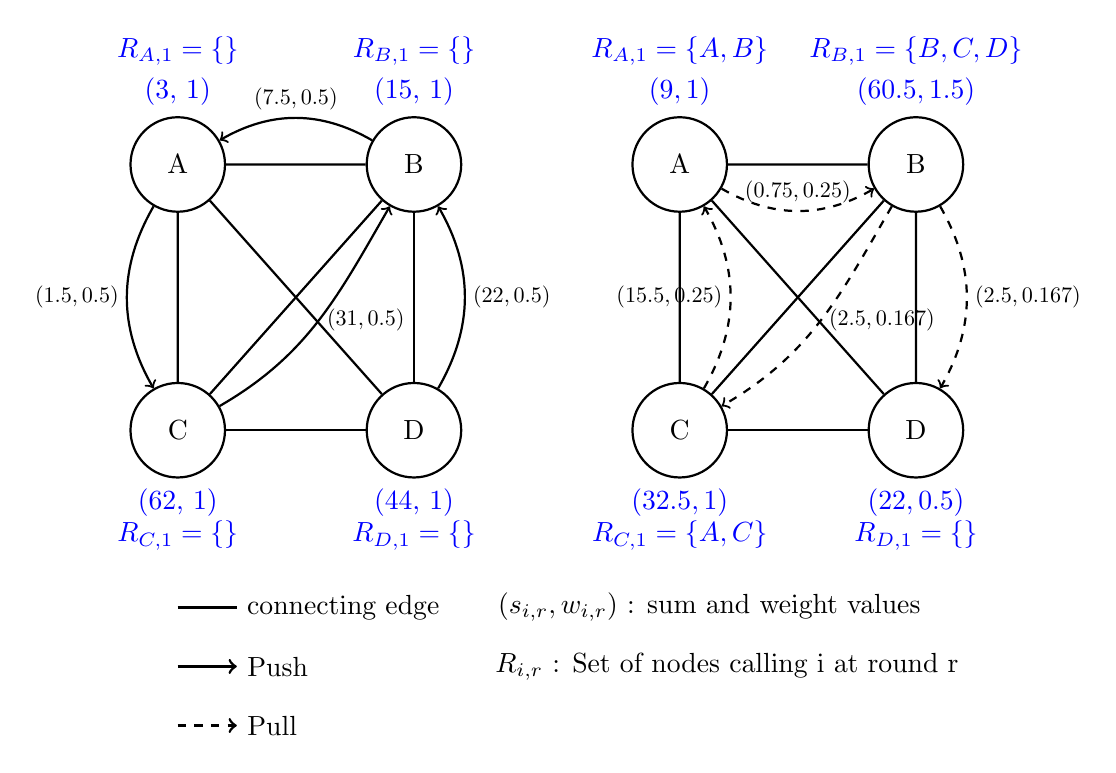
\begin{tikzpicture}[scale=0.75, thick, main node/.style={circle, draw, minimum size=1.2cm}]

    % First graph
    \node[main node] (A1) at (-1,4.5) {A};
    \node[main node] (B1) at (3,4.5) {B};
    \node[main node] (C1) at (-1,0) {C};
    \node[main node] (D1) at (3,0) {D};
    
    \node[above, color=blue] at (A1.north) {(3, 1)};
    \node[above, color=blue] at (B1.north) {(15, 1)};
    \node[below, color=blue] at (C1.south) {(62, 1)};
    \node[below, color=blue] at (D1.south) {(44, 1)};

    \node[above, color=blue] at (-1,6) {$R_{A,1}=\{\}$};
    \node[above, color=blue] at (3,6) {$R_{B,1}=\{\}$};
    \node[above, color=blue] at (-1,-2.2) {$R_{C,1}=\{\}$};
    \node[above, color=blue] at (3,-2.2) {$R_{D,1}=\{\}$};

     \node[above, color=blue] at (7.5,6) {$R_{A,1}=\{A, B\}$};
    \node[above, color=blue] at (11.5,6) {$R_{B,1}=\{B, C, D\}$};
    \node[above, color=blue] at (7.5,-2.2) {$R_{C,1}=\{A, C\}$};
    \node[above, color=blue] at (11.5,-2.2) {$R_{D,1}=\{\}$};
    
    \draw (A1) -- (B1);
    \draw (A1) -- (C1);
    \draw (A1) -- (D1);
    \draw (B1) -- (C1);
    \draw (B1) -- (D1);
    \draw (C1) -- (D1);

    % Second graph
    \node[main node] (A2) at (7.5,4.5) {A};
    \node[main node] (B2) at (11.5,4.5) {B};
    \node[main node] (C2) at (7.5,0) {C};
    \node[main node] (D2) at (11.5,0) {D};
    
    \node[above, color=blue] at (A2.north) {$(9, 1)$};
    \node[above, color=blue] at (B2.north) {$(60.5, 1.5)$};
    \node[below, color=blue] at (C2.south) {$(32.5, 1)$};
    \node[below, color=blue] at (D2.south) {$(22, 0.5)$};
    
    \draw (A2) -- (B2);
    \draw (A2) -- (C2);
    \draw (A2) -- (D2);
    \draw (B2) -- (C2);
    \draw (B2) -- (D2);
    \draw (C2) -- (D2);

    \draw[->] (A1) to[out=240, in=120] node[left, scale=0.8] {$(1.5, 0.5)$} (C1);
    \draw[->] (B1) to[out=150, in=30] node[above, scale=0.8] {$(7.5, 0.5)$} (A1);
    \draw[->] (C1) to[out=30, in=240] node[right, scale=0.8] {$(31, 0.5)$} (B1);
    \draw[->] (D1) to[out=60, in=300] node[right,scale=0.8] {$(22, 0.5)$} (B1);


    
    %\draw[dashed, ->] (C1) to[out=60, in=300] node[right] {$\frac{l_{C}-l_{A}}{2}$} (A1);
    %\draw[dashed, ->] (A1) to[out=330, in=210] node[right] {$\frac{l_{C}-l_{A}}{2}$} (B1);
    

    
    \draw[dashed, ->] (C2) to[out=60, in=300] node[left, scale=0.8 ] {$(15.5, 0.25)$} (A2);
    \draw[dashed, ->] (A2) to[out=-30, in=210] node[above, scale=0.8] {$(0.75, 0.25)$} (B2);
    \draw[dashed, ->] (B2) to[out=240, in=30] node[right, scale=0.8] {$(2.5,0.167)$} (C2);
    \draw[dashed, ->] (B2) to[out=300, in=60] node[right, scale=0.8] {$(2.5,0.167)$} (D2);

    % Legend in the middle below the graphs
    \begin{scope}[shift={(3,-3)}]
        % Horizontal line
        \draw (-4,0) -- (-3,0) node[right] {connecting edge};
        % Long right arrow
        \draw[->, line width=1pt] (-4,-1) -- (-3,-1) node[right] {Push};
        % Long right dashed arrow
        \draw[->, dashed, line width=1pt] (-4,-2) -- (-3,-2) node[right] {Pull};
        
        % Load notation
        \node at (5,0) {$(s_{i,r}, w_{i,r})$ : sum and weight values};
        \node at (5.3,-1) {$R_{i,r}$ : Set of nodes calling i at round r};
    \end{scope}

\end{tikzpicture}}
    \caption{Push-Pull Sum: push and pull actions}
    \label{fig:examplePPSSetting}
\end{figure}

The example in figure \ref{fig:examplePPSSetting} illustrates a execution of the Push-Pull Sum algorithm on a Complete graph $K_4$ with four nodes labeled \textit{A, B, C} and \textit{D}. Each node is initially assigned a sum and a weight value. The undirected graph represents the network topology. The nodes are connected by edges. The solid directed edges depict the push operations and the dashed directed edges visualize the pull operations. Each node maintains a set $R_{i,r}$ where $i$ is the node ID and $r$ is the round being examined. The load of the node is calculated by $\frac{s_{i,r}}{w_{i,r}}$. The example depicts the first round of a execution of the Push-Pull Sum algorithm. The push and pull operations are distinct. The left-hand side of figure \ref{fig:examplePPSSetting} depicts the behavior of the nodes while executing the push operations, while the right side illustrates the pull operations. During the push phase, each node randomly selects a neighbor to transfer load to. In this example:

\begin{itemize}
    \item Node $A$ selects node $C$ and pushes half of its sum and weight to both node $C$ and itself. (Self-loops are omitted from the figure for readability.)
    \item Node $B$ selects node $A$ as its trading partner.
    \item Nodes $C$ and $D$ push their values to node $B$ and themselves.
\end{itemize}

Given the push operations for each node, the set $R_{i,r}$ is computed. Since node $B$ pushed load to node $A$ and node $A$ pushed load to itself, the requesting nodes for node $A$ are $R_{A,1}=\{A,B\}$. The updated sum and weight values after the push phase can be inspected on the right-hand side of figure \ref{fig:examplePPSSetting}.

Following the push actions, each node proceeds with the \textit{ResponseData}-procedure, executing the pull phase. Each node in $R_{i,1}$ receives a response based on the respective pull values. Since node $A$ has two nodes in its set $R_{A,1}$, it responds to both node $B$ and itself with $\left(\frac{\frac{3}{2}}{2}, \frac{\frac{1}{2}}{2}\right)$, as indicated by a dashed directed edge. Similarly, the remaining nodes \textit{B, C, and D} execute their pull operations. Following the push and pull operations, the nodes update their sum and weight values. The state of the network after round one is depicted in figure \ref{fig:examplePPSResult}. The MSE at the beginning of round 1 is $542.50$. After applying one round of the Push-Pull Sum algorithm, the MSE is reduced to $63.49$.

\begin{figure}
    \centering
    \scalebox{0.75}{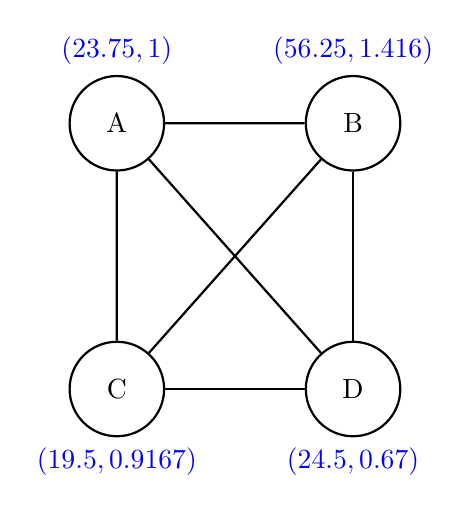
\begin{tikzpicture}[scale=0.75, thick, main node/.style={circle, draw, minimum size=1.2cm}]

    % First graph
    \node[main node] (A1) at (-1,4.5) {A};
    \node[main node] (B1) at (3,4.5) {B};
    \node[main node] (C1) at (-1,0) {C};
    \node[main node] (D1) at (3,0) {D};
    
    \node[above, color=blue] at (A1.north) {$(23.75,1)$};
    \node[above, color=blue] at (B1.north) {$(56.25, 1.416)$};
    \node[below, color=blue] at (C1.south) {$(19.5, 0.9167)$};
    \node[below, color=blue] at (D1.south) {$(24.5, 0.67)$};
    
    \draw (A1) -- (B1);
    \draw (A1) -- (C1);
    \draw (A1) -- (D1);
    \draw (B1) -- (C1);
    \draw (B1) -- (D1);
    \draw (C1) -- (D1);

\end{tikzpicture}}
    \caption{Push-Pull Sum: setting after round 1}
    \label{fig:examplePPSResult}
\end{figure}

\section{Continuous Single-Proposal Deal-Agreement-Based Algorithm}\label{sec:singleproposalDAB}
The Continuous Single-Proposal Deal-Agreement-Based algorithm proposed by Dinitz et al. \cite{Dinitz2023DAB} is unlike the Push-Pull Sum algorithm, not a diffusion-based algorithm. The goal of load balancing is achieved based on deterministic deal agreements, where one node proposes a load to one neighboring node, and the neighboring node accepts the transfer proposal either fully or partially. Dinitz et al. proved that the algorithm has the anytime property, meaning it never worsens the state of the network during execution. Their study examined the algorithm in a dynamic setting, where each node has access to a set of neighboring nodes, including the node's loads. The algorithm is divided into three phases: \textit{proposal}, \textit{deal}, and \textit{summary}. In the \textit{proposal}-phase, each node $u$ identifies its minimally loaded neighbor \textit{v} and sends a proposal to that neighbor if $v$ has a lower load. The proposal is of value:
\begin{align}
    \frac{load_{r}(u)-load_{r}(v)}{2}    
\end{align}
which is labeled as a \textit{fair} proposal. Since the load transfer is fair, the resulting load of $u$ is not lower than that of $v$. $load_{r}(u)$ represents the load of node $u$ at round $r$. In the \textit{deal}-phase, nodes evaluate the deals proposed to them. A node accepts the deal of the node that proposes the maximal load transfer. The actual transfer happens, and the nodes update their loads. Finally, in the \textit{summary}-phase, each node informs their neighbors regarding their updated load values. \cite{Dinitz2023DAB}

\renewcommand{\algorithmicrequire}{\textbf{Input:}}
\renewcommand{\algorithmicensure}{\textbf{Output:}}
\begin{algorithm}
\caption{Continuous Single-Proposal Deal-Agreement-Based protocol}\label{alg:DAB}
\begin{algorithmic}[1]
\Require An undirected graph $G=(V,E,load)$
\Ensure A load state with discrepancy at most $\epsilon$ on $G$
\For{$r=1$ and on}
\For{every node u}
\State Find a neighbor, $v$, with the minimal load
\If{$load_{r}(u) - load_{r}(v)>0$}
\State $u$ sends to $v$ a transfer proposal of value $(load_{r}(u)-load_{r}(v))/2$
\EndIf
\EndFor

\For{every node $u$}
\If{there is at least one transfer proposal to $u$}
\State Find a neighbor, $w$, proposing to $u$ the maximal transfer
\State Node $u$ makes a deal: informs node $w$ on accepting its proposal
\State The actual transfer from $w$ to $u$ is executed 
\EndIf
\EndFor

\For{every node $u$}
\State Node $u$ sends the updated value of its load to its neighbors
\EndFor
\EndFor
\end{algorithmic}
\end{algorithm}


The potential for a node $u$ is defined as:
\begin{align}
    p(u) = (load(u)-L_{avg})^{2}    
\end{align}
where $L_{avg}$ represents the current load average in the network. The potential for the graph $p(G)$ is defined as:
\begin{align}
    p(G)=\sum_{i\in V}{p(i)},   
\end{align}
which is the sum of the potentials of each node in the graph G. Any fair load transfer of load $l$ decreases the potential of the graph by at least $2l^{2}$. As a result of any round $r$ of the Continuous Single-Proposal Deal-Agreement-Based algorithm, the graph potential decreases by at least $\frac{K^{2}_r}{2D_r}$, where $K$ is the initial discrepancy and $D$ is a bound for the graph diameter. \cite{Dinitz2023DAB}

The Single-Proposal Deal-Agreement-Based load balancing algorithm struggles to reduce the MSE as rapidly as the Push-Pull Sum algorithm for dense graphs like the Complete graph, the Lollipop graph with a large clique size, and the Ring of Cliques with a large clique size. This limitation arises because each node looks for the minimally loaded partner for a load transfer. For a Complete graph, the minimally loaded load partner is the same node with loads of $L_{min}$ (the minimally loaded node in the network). This causes each node that does not hold $L_{min}$ to propose to the same node, which then evaluates the proposals and accepts exactly one transfer proposal, namely the maximal one. This situation is described in detail in the appendix in section \ref{sec:struggleDAB} using an example. A similar scenario occurs in the Ring of Cliques and the Lollipop graph. However, in the Ring of Cliques, nodes do not all propose to the same minimally loaded neighbor, instead, they propose to the least-loaded neighbor within their respective cliques. For the Lollipop graph, the nodes in the path graph balance their loads more quickly than the nodes in the clique, which is a bottleneck in this scenario. For the Torus Grid and the Ring graph, the Deal-Agreement-Based algorithm performs better in reducing the error compared to the Push-Pull Sum algorithm. In these scenarios, the proposals are more evenly distributed among nodes due to the lower density of the graphs. The Star graph is an exception to this case, since we have a similar bottleneck as in the Complete graph, as the central node is the common neighbor for each leaf, thus each leaf proposes a load to the central node. The central node can accept only one proposal. Again, an example of this is provided in the appendix in section \ref{sec:struggleDAB}.

\subsection{Example}\label{subsec:exampleDAB}
 \begin{figure}
    \centering
    \scalebox{0.75}{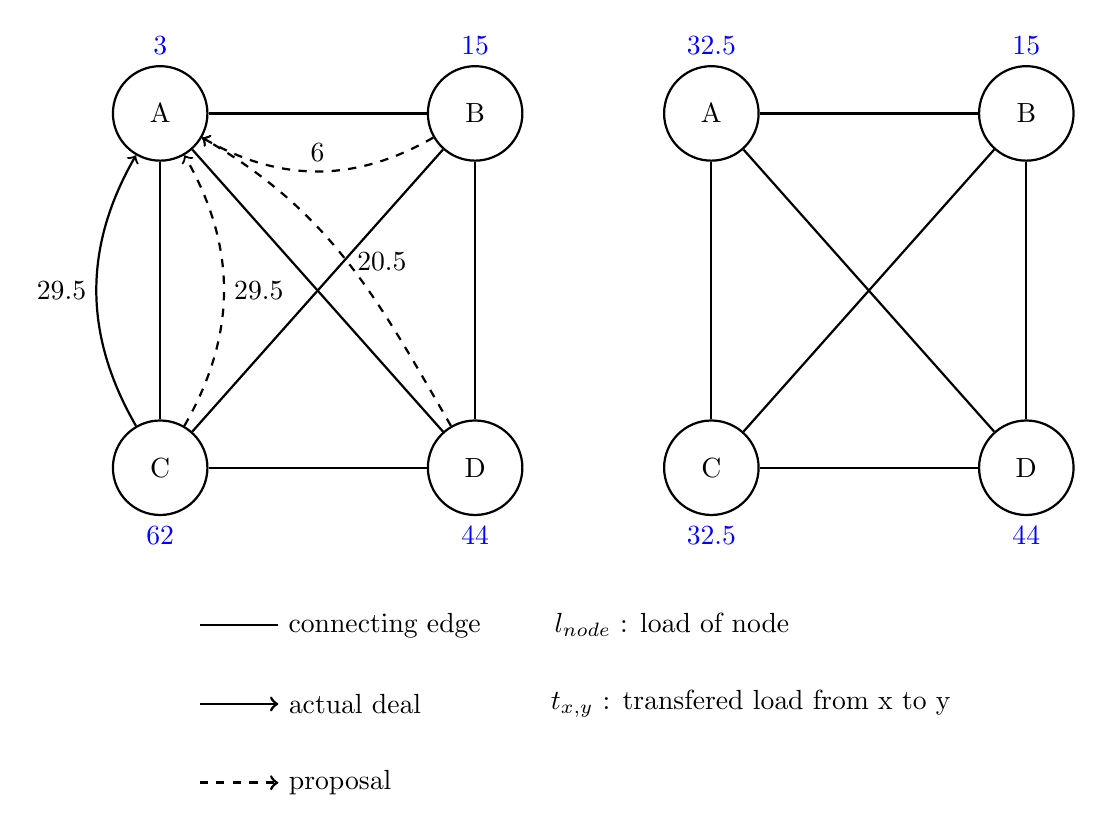
\begin{tikzpicture}[ thick, main node/.style={circle, draw, minimum size=1.2cm}]

    % First graph
    \node[main node] (A1) at (0.5,4.5) {A};
    \node[main node] (B1) at (4.5,4.5) {B};
    \node[main node] (C1) at (0.5,0) {C};
    \node[main node] (D1) at (4.5,0) {D};
    
    \node[above, color=blue] at (A1.north) {3};
    \node[above, color=blue] at (B1.north) {15};
    \node[below, color=blue] at (C1.south) {62};
    \node[below, color=blue] at (D1.south) {44};
    
    \draw (A1) -- (B1);
    \draw (A1) -- (C1);
    \draw (A1) -- (D1);
    \draw (B1) -- (C1);
    \draw (B1) -- (D1);
    \draw (C1) -- (D1);

    % Second graph
    \node[main node] (A2) at (7.5,4.5) {A};
    \node[main node] (B2) at (11.5,4.5) {B};
    \node[main node] (C2) at (7.5,0) {C};
    \node[main node] (D2) at (11.5,0) {D};
    
    \node[above, color=blue] at (A2.north) {32.5};
    \node[above, color=blue] at (B2.north) {15};
    \node[below, color=blue] at (C2.south) {32.5};
    \node[below, color=blue] at (D2.south) {44};
    
    \draw (A2) -- (B2);
    \draw (A2) -- (C2);
    \draw (A2) -- (D2);
    \draw (B2) -- (C2);
    \draw (B2) -- (D2);
    \draw (C2) -- (D2);

    \draw[->] (C1) to[out=120, in=240] node[left] {$29.5$} (A1);
    \draw[dashed, ->] (C1) to[out=60, in=300] node[right] {$29.5$} (A1);
    \draw[dashed, ->] (B1) to[out=210, in=330] node[above] {$6$} (A1);
    \draw[dashed, ->] (D1) to[out=120, in=330] node[right] {$20.5$} (A1);

    % Legend in the middle below the graphs
    \begin{scope}[shift={(3,-2)}]
        % Horizontal line
        \draw (-2,0) -- (-1,0) node[right] {connecting edge};
        % Long right arrow
        \draw[->, line width=1pt] (-2,-1) -- (-1,-1) node[right] {actual deal};
        % Long right dashed arrow
        \draw[->, dashed, line width=1pt] (-2,-2) -- (-1,-2) node[right] {proposal};
        
        % Load notation
        \node at (4,0) {$l_{node}$ : load of node};
        \node at (5,-1) {$t_{x,y}$ : transfered load from x to y};
    \end{scope}

\end{tikzpicture}}
    \caption{Deal-Agreement-Based: initial setup and setup after round 1}
    \label{fig:DABExampleAlgo}
 \end{figure}
Figure \ref{fig:DABExampleAlgo} illustrates two settings. The left-hand side of the figure depicts the initial state and the right-handside illustrates the state after one round of execution. The setting is the same as in the example above for the Push-Pull Sum, with the difference that each node is assigned a load value, instead of sum and weight values. The dashed directed edges represent transfer proposals from one node to another, while solid directed edges indicate actual load transfers. The network consists of four nodes, labeled \textit{A, B, C,} and \textit{D}. Each node identifies its least-loaded neighbor as a potential transfer recipient. Nodes \textit{B, C} and \textit{D} determine node $A$ as their minimal loaded neighbors. Node $A$ identifies node $B$ as the neighbor with the minimal load in its neighborhood, however node $B$ has more load than node $A$, so node $A$ does not send an transfer proposal to node $B$. As a result, nodes \textit{B, C} and \textit{D} each send a transfer proposal of value $\frac{(load_r(i)-load_r(A))}{2}$ to node $A$, where $i \in \{B,C,D\}$. Node $A$ evaluates the proposal and accepts node $C$'s transfer proposal, as node $C$ proposes the largest amount of load, namely $29.5$. The actual transfer happens and $29.5$ of loads are transfered from node $C$ to node $A$. The right-hand side of figure \ref{fig:DABExampleAlgo} shows the state of the network after round 1 of executing the Deal-Agreement-Based algorithm. Node $A$ and $C$ each have equal loads of $32.5$, the loads of nodes $B$ and $D$ remain unchanged. The MSE at the beginning of round 1 is at $542.5$. After executing the first round of the algorithm the MSE decreases to a value of $107.375$, which is approximately one-fifth of the initial MSE.

\section{Adaptive Threshold Push-Pull Sum Algorithm}\label{sec:adaptivethresholdPPS}
The Adaptive Threshold Push-Pull Sum algorithm is composed of key elements from both the Push-Pull Sum and Single-Proposal Deal-Agreement-Based algorithms, extended by the idea of adaptive thresholding. The Adaptive Threshold Push-Pull Sum consists of different procedures. In the \textit{CheckThresholdsRequestData}, each node $u$ chooses a subset $RN_{u,r}$ with:
\begin{align}
    RN_{u,r} \subseteq neighborhood_{u}, |RN_{u,r}|=\lceil \log_{2}{(|neighborhood_{u}|)} \rceil
\end{align}
random neighbors. This increases the likelihood of selecting a well-suited neighbor for a load transfer. Selecting only one random neighbor lowers the chance to find an optimal or good neighbor to execute a load transfer. The load difference between the node $u$ and the nodes in $RN_{u,r}$ is computed and checked against a threshold $\theta$. The threshold is computed in the \textit{CalculateThresholds}-procedure. The threshold $\theta$ is calculated as:
\begin{align}
    \theta = k*\sqrt{MSE_{r-1}}    
\end{align}
where $k$ is some factor to adjust the sensitivity of the threshold. A larger $k$ makes the threshold more sensitive, meaning that fewer nodes are eligible for load transfer, allowing only significant load transfer. Respectively, a smaller $k$ makes the threshold less strict, so, more nodes are eligible for load transfers. This condition ensures that only load transfers with meaningful impact happen, and load transfers between nodes with low impact on the balance of the network are avoided. The first eligible node in $RN_{u,r}$ that exceeds the threshold receives the sum of value $(\frac{s_{i,r}}{2})$ and the weight of value $(\frac{w_{i,r}}{2})$. The \textit{ResponseData} and the \textit{Aggregate}-procedure are directly adapted from the Push-Pull Sum algorithm. The way the loads are distributed, is directly taken from the Push-Pull Sum algorithm and extended by an adaptive threshold mechanism. Like the Single-Proposal Deal-Agreement-Based algorithm, the Adaptive Threshold Push-Pull Sum algorithm employs conditional load transfers, but with a threshold $\theta$ instead of requiring a strictly positive load difference. Instead of initiating a load transfer with the maximally proposing node, the Adaptive Threshold Push-Pull Sum algorithm orders the nodes to initiate a load transfer with the first node proposing load (the first node, where the load difference passes the threshold). The reason for that is to reduce computational overhead by avoiding that each node looks through its whole set $RN$ and is required to evaluate each proposal. So the first node proposing a load transfer is accepted as a transfer partner.

Although formally not shown, the Adaptive Threshold Push-Pull Sum algorithm is expected to hold the mass conservation property, as it converged to the correct ground truth in all experiment settings, similar to the Push-Pull Sum algorithm. Also, given that the push and pull mechanisms are directly adapted, these operations are the only operations that let nodes transfer or receive nodes in the algorithm. The Adaptive Threhsold Push-Pull Sum algorithm is an stochastic algorithm as it inherits its stochastic nature from the Push-Pull Sum algorithm, by choosing a subset of neighbors randomly.

\begin{algorithm}
    \caption{Adaptive Threshold Push-Pull Sum algorithm}\label{alg:PPS}
    \begin{algorithmic}[1]
    \Procedure{CalculateThresholds}{}
    \State $\theta \leftarrow k * \sqrt{MSE_{r-1}}$ 
    \EndProcedure
    \Procedure{CheckTresholdRequestData}{}
    \State $RN_{u,r} \leftarrow$ choose $\lceil \log_{2}{(|neighborhood(u)|)} \rceil$ random neighbor
    \For{every node $v_{i} \in RN_{u,r}$}
    \State $\Delta_{u, v_{i}} \leftarrow |(load(u) - load(v_{i}))|$
    \If{$\Delta_{u,v} > \theta$}
    \State Send $(\frac{s_{u,r}}{2}, \frac{w_{u,r}}{2})$ to first node v fulfilling condition and the node $u$ itself
    \EndIf
    \EndFor
    \EndProcedure
    \Procedure{ResponseData}{}
    \State $R_{u,r} \leftarrow$ Set of the nodes calling $u$ at a round $r$
    \For{\textbf{all} $i \in R_{u,r}$}
    \State Reply to i with $\left( \frac{\frac{s_{u,r}}{2}}{|R_{u,r}|}, \frac{\frac{w_{u,r}}{2}}{|R_{u,r}|} \right)$
    \EndFor
    \EndProcedure
    \Procedure{Aggregate}{}
    \State $M_{u,t} \leftarrow \{(s_{m}, w_{m})\}$ messages sent to $u$ at a round $r-1$
    \State $s_{u,t} \leftarrow \sum_{m \in M_{u,r}}^{}s_{m}, w_{u,r} \leftarrow\sum_{m \in M_{u,r}}^{}w_{m}$
    \State $load(u) \leftarrow \frac{s_{u,r}}{w_{u,r}}$
    \EndProcedure
    \end{algorithmic}
    \end{algorithm}

\subsection{Example}\label{subsec:exampleAdaptiveThresholdPPS}
\begin{figure}
    \centering
    \scalebox{0.75}{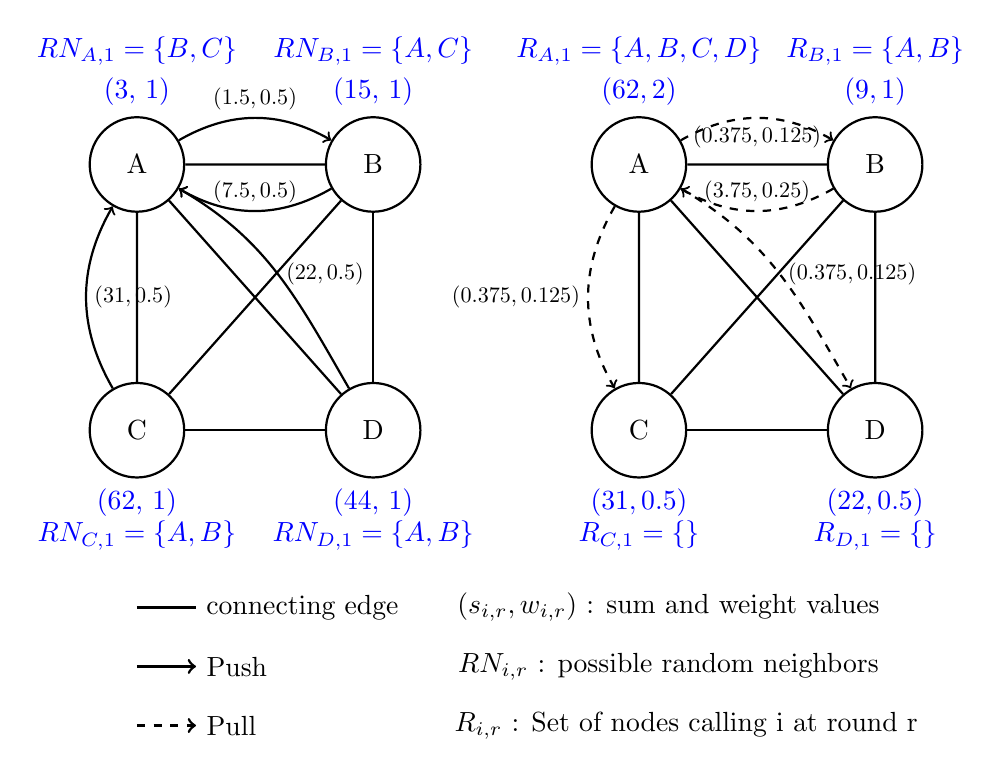
\begin{tikzpicture}[scale=0.75, thick, main node/.style={circle, draw, minimum size=1.2cm}]

    % First graph
    \node[main node] (A1) at (-1,4.5) {A};
    \node[main node] (B1) at (3,4.5) {B};
    \node[main node] (C1) at (-1,0) {C};
    \node[main node] (D1) at (3,0) {D};
    
    \node[above, color=blue] at (A1.north) {(3, 1)};
    \node[above, color=blue] at (B1.north) {(15, 1)};
    \node[below, color=blue] at (C1.south) {(62, 1)};
    \node[below, color=blue] at (D1.south) {(44, 1)};

    \node[above, color=blue] at (-1,6) {$RN_{A,1}=\{B,C\}$};
    \node[above, color=blue] at (3,6) {$RN_{B,1}=\{A,C\}$};
    \node[above, color=blue] at (-1,-2.2) {$RN_{C,1}=\{A,B\}$};
    \node[above, color=blue] at (3,-2.2) {$RN_{D,1}=\{A,B\}$};

     \node[above, color=blue] at (7.5,6) {$R_{A,1}=\{A, B, C, D\}$};
    \node[above, color=blue] at (11.5,6) {$R_{B,1}=\{A, B\}$};
    \node[above, color=blue] at (7.5,-2.2) {$R_{C,1}=\{\}$};
    \node[above, color=blue] at (11.5,-2.2) {$R_{D,1}=\{\}$};
    
    \draw (A1) -- (B1);
    \draw (A1) -- (C1);
    \draw (A1) -- (D1);
    \draw (B1) -- (C1);
    \draw (B1) -- (D1);
    \draw (C1) -- (D1);

    % Second graph
    \node[main node] (A2) at (7.5,4.5) {A};
    \node[main node] (B2) at (11.5,4.5) {B};
    \node[main node] (C2) at (7.5,0) {C};
    \node[main node] (D2) at (11.5,0) {D};
    
    \node[above, color=blue] at (A2.north) {$(62, 2)$};
    \node[above, color=blue] at (B2.north) {$(9, 1)$};
    \node[below, color=blue] at (C2.south) {$(31, 0.5)$};
    \node[below, color=blue] at (D2.south) {$(22, 0.5)$};
    
    \draw (A2) -- (B2);
    \draw (A2) -- (C2);
    \draw (A2) -- (D2);
    \draw (B2) -- (C2);
    \draw (B2) -- (D2);
    \draw (C2) -- (D2);

    \draw[->] (A1) to[out=30, in=150] node[above, scale=0.8] {$(1.5, 0.5)$} (B1);
    \draw[->] (B1) to[out=210, in=-30] node[above, scale=0.8] {$(7.5, 0.5)$} (A1);
    \draw[->] (C1) to[out=120, in=240] node[right, scale=0.8] {$(31, 0.5)$} (A1);
    \draw[->] (D1) to[out=120, in=-30] node[right, scale=0.8] {$(22, 0.5)$} (A1);


    
    %\draw[dashed, ->] (C1) to[out=60, in=300] node[right] {$\frac{l_{C}-l_{A}}{2}$} (A1);
    %\draw[dashed, ->] (A1) to[out=330, in=210] node[right] {$\frac{l_{C}-l_{A}}{2}$} (B1);
    

    
    \draw[dashed, ->] (A2) to[out=30, in=150] node[below, scale=0.8] {$(0.375, 0.125)$} (B2);
     \draw[dashed, ->] (A2) to[out=240, in=120] node[left, scale=0.8] {$(0.375, 0.125)$} (C2);
     \draw[dashed, ->] (A2) to[out=-30, in=120] node[right, scale=0.8] {$(0.375,0.125)$} (D2);
      \draw[dashed, ->] (B2) to[out=210, in=-30] node[above, scale=0.8] {$(3.75,0.25)$} (A2);

    % Legend in the middle below the graphs
    \begin{scope}[shift={(3,-3)}]
        % Horizontal line
        \draw (-4,0) -- (-3,0) node[right] {connecting edge};
        % Long right arrow
        \draw[->, line width=1pt] (-4,-1) -- (-3,-1) node[right] {Push};
        % Long right dashed arrow
        \draw[->, dashed, line width=1pt] (-4,-2) -- (-3,-2) node[right] {Pull};
        
        % Load notation
        \node at (5,0) {$(s_{i,r}, w_{i,r})$ : sum and weight values};
        \node at (5,-1) {$RN_{i,r}$ : possible random neighbors};
        \node at (5.3,-2) {$R_{i,r}$ : Set of nodes calling i at round r};
    \end{scope}

\end{tikzpicture}}
    \caption{Adaptive Threshold Push-Pull Sum: push and pull actions}
    \label{fig:ATPPSExampleSetting}
\end{figure}

Figure \ref{fig:ATPPSExampleSetting} depicts a similar setting as described in section \ref{subsec:examplePPS}. According to the Adaptive Threshold Push-Pull Sum algorithm, each node chooses $\lceil \log_{2}{(|neighborhood_{i}|)} \rceil$ neighbors. For this setting, each node chooses two neighbors, which are added to the set $RN_{i,1}$ for each node $i$. For instance, node $A$ computes $RN_{A,1}$ as $\{B,C\}$. The load differences between node $A$ and nodes $B$ and $C$ are computed. In this example, $k$ is set to $0.01$, thus the threshold $\theta$ is given by $0.01*\sqrt{542.5} \approx 0.23$. Since both load differences between nodes $A$ and $B$ and nodes $A$ and $C$ exceed this threshold, both nodes are eligible to propose a load transfer with node $A$. In this scenario, node $A$ selects node $B$ as a transfer partner and pushes half of its sum $1.5$ and weight $0.5$ to node $B$ and itself. This process is repeated for each node accordingly. Similar to the example in section \ref{subsec:examplePPS}, the nodes then execute the pull operation. The result is depicted in figure \ref{fig:ATPPSExampleResult}. The MSE dropped from $542.5$ initially to $251.86$. The error reduction depends on the sensitivity factor $k$. If $k$ is set to 1, the load transfer between node $A$ and $B$ would not have happened. Instead, nodes $A$ and $C$ would have exchanged loads, leading to a larger impact on the balance of the network. 

\begin{figure}
    \centering
    \scalebox{0.75}{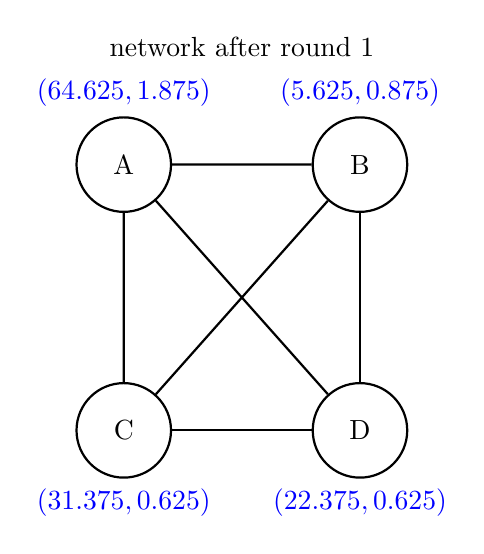
\begin{tikzpicture}[scale=0.75, thick, main node/.style={circle, draw, minimum size=1.2cm}]

    % First graph
    \node[main node] (A1) at (-1,4.5) {A};
    \node[main node] (B1) at (3,4.5) {B};
    \node[main node] (C1) at (-1,0) {C};
    \node[main node] (D1) at (3,0) {D};
    
    \node[above, color=blue] at (A1.north) {$(64.625,1.875)$};
    \node[above, color=blue] at (B1.north) {$(5.625, 0.875)$};
    \node[below, color=blue] at (C1.south) {$(31.375, 0.625)$};
    \node[below, color=blue] at (D1.south) {$(22.375, 0.625)$};
    
    \draw (A1) -- (B1);
    \draw (A1) -- (C1);
    \draw (A1) -- (D1);
    \draw (B1) -- (C1);
    \draw (B1) -- (D1);
    \draw (C1) -- (D1);

    \node at (1,6.5) {network after round 1};


\end{tikzpicture}}
    \caption{Adaptive Threshold Push-Pull Sum: setting after round 1}
    \label{fig:ATPPSExampleResult}
\end{figure}
\subsection{Aspired Outcome}\label{subsec:aspiredOutcomeAdaptiveThresholdPPS}

Considering the simulation results presented in \cite{Bayazitoglu}, the discrepancy between the MSE reduction abilities per round for the different topologies shows that the algorithms perform either very well or mediocre to bad. The motivation behind designing the Adaptive Threshold Push-Pull Sum algorithm was to find a compromise solution that enhances adaptability across various network topologies.

The final results of the first load balancing step can be taken from table \ref{tab:overviewExamples}. The Push-Pull Sum algorithm shows the lowest MSE after round one, followed by the Deal-Agreement-Based algorithm and the Adaptive Threshold Push-Pull Sum algorithm. A small $k$ value was used for demonstrative purposes (as the simulations in chapter \ref{chap:simulationoutcomes} were conducted with small $k$ values). A higher k value would have a greater impact in the first round. In section \ref{chap:simulationoutcomes}, we will see that the Adaptive Threshold Push-Pull Sum algorithm proceeds to enhance in reducing error in later rounds, as the MSE and thus the thresholds adjust.

\begin{table}
\centering
\begin{tabular}{|c|c|c|c|c|}
\hline
 & \textbf{Initial} & \textbf{Dinitz et al.} & \textbf{Nugroho et al.} & \textbf{Bayazitoglu} \\ \hline
\textbf{Node A}  & 3      & 32.5    & (23.75, 1) = 23.75     & (64.625, 1.875) = 34.47 \\ \hline
\textbf{Node B}  & 15     & 15      & (56.25, 1.416) = 39.72 & (5.625, 0.875) = 6.43   \\ \hline
\textbf{Node C}  & 62     & 32.5    & (19.5, 0.9167) = 21.27 & (31.375, 0.625) = 50.2  \\ \hline
\textbf{Node D}  & 44     & 44      & (24.5, 0.67) = 36.57   & (22.375, 0.625) = 35.8  \\ \hline
\textbf{MSE} & 542.50 & 107.375 & 63.49                  & 251.86                  \\ \hline
\end{tabular}
\caption{State of loads after one round}
\label{tab:overviewExamples}
\end{table}